\documentclass[12pt, letterpaper, preprint]{aastex}
\usepackage{hyperref}
\usepackage{color}
%%% This file is generated by the Makefile.
\newcommand{\giturl}{\url{https://github.com/changhoonhahn/centralMS}}
\newcommand{\githash}{9119283}\newcommand{\gitdate}{2019-04-05}\newcommand{\gitauthor}{changhoonhahn}


% typesetting shih
\linespread{1.08} % close to 10/13 spacing
\setlength{\parindent}{1.08\baselineskip} % Bringhurst
\setlength{\parskip}{0ex}
\let\oldbibliography\thebibliography % killin' me.
\renewcommand{\thebibliography}[1]{%
  \oldbibliography{#1}%
  \setlength{\itemsep}{0pt}%
  \setlength{\parsep}{0pt}%
  \setlength{\parskip}{0pt}%
  \setlength{\bibsep}{0ex}
  \raggedright
}
\setlength{\footnotesep}{0ex} % seriously?

\newcommand\tab[1][1cm]{\hspace*{#1}}
\newcommand{\todo}[1]{{\bf \textcolor{red}{#1}}}
\newcommand{\beq}{\begin{equation}}
\newcommand{\eeq}{\end{equation}}
\newcommand{\overbar}[1]{\mkern 1.5mu\overline{\mkern-1.5mu#1\mkern-1.5mu}\mkern 1.5mu}
\newcommand{\avgSFR}{\overline{\raisebox{0pt}[1.2\height]{SFR}}}
\newcommand{\SFR}{\mathrm{SFR}}
\newcommand{\fq}{f_\mathrm{Q}}
\newcommand{\fqcen}{f_\mathrm{Q}^\mathrm{cen}}
\newcommand{\zinit}{z_\mathrm{initial}}
\newcommand{\taucen}{\tau_\mathrm{Q}^\mathrm{cen}}
\newcommand{\bitem}{\begin{itemize}}
\newcommand{\eitem}{\end{itemize}}

\begin{document}\sloppy\sloppypar\frenchspacing

%\title{Central Galaxies on the Main Sequence} 
\title{Star Formation Main Sequence in a Hierarchical Universe} 
\date{\texttt{DRAFT~---~\githash~---~\gitdate~---~NOT READY FOR DISTRIBUTION}}
\author{ChangHoon~Hahn\altaffilmark{1}, 
Jeremy L.~Tinker\altaffilmark{2}, 
Andrew R.~Wetzel\altaffilmark{3,4,5}}
\altaffiltext{1}{Lawrence Berkeley National Laboratory, 1 Cyclotron Road, Berkeley, CA 94720}
\altaffiltext{3}{Center for Cosmology and Particle Physics, Department of Physics, New York University, 4 Washington Place, New York, NY 10003}
\altaffiltext{4}{TAPIR, California Institute of Technology, Pasadena, CA USA}
\altaffiltext{5}{Carnegie Observatories, Pasadena, CA USA}
\altaffiltext{6}{Department of Physics, University of California, Davis, CA USA}
\email{changhoon.hahn@lbl.gov}

\begin{abstract}
    \todo{motivation, methodology, impact.}
    
    In observations star forming galaxies form a tight $log\;M_*$ to $log\;SFR$ 
    relation referred to as the {\em star formation main sequence} (SFMS) out to $z\sim2$. 
    Beyond the evolution ``along'' this SFMS, however, the star formation histories of star 
    forming galaxies have not been precisely characterized. 
    The SFH of these galaxies govern SMF, SFMS, and also observed constraints on the stellar mass to halo mass
    relation. 

    By combining high-resolution cosmological $N$-body simulation with observed evolutionary 
    trends of SF galaxies, we construct a model that tracks the evolution of star forming 
    central galaxies over the redshift $z < 1$. Comparing this model 

    Observations find a remarkably small scatter in the stellar mass to halo mass relation. 
    Somehow the star formation histories of galaxies must 
    
    According to observations, star forming galaxies form a tight $log\;M_*$ to $log\;SFR$ 
    relation referred to as the ``star formation main sequence'' out to $z\sim2$. 
\end{abstract}
\keywords{methods: numerical -- galaxies: clusters: general -- 
galaxies: groups: general -- galaxies: evolution -- galaxies: haloes -- 
galaxies: star formation -- cosmology: observations.}


{\bf Checklist} 
\bitem
\item Check the correlation between halo growth rate with different $t_{delay}$ and $\delta t_{abias}$ with the total halo growth rate between $z \sim 0$ and $z \sim 1$. 
\eitem 

\section{Introduction}
\bitem 
\item Motivate why we think SF galaxies evolve along the main sequence  
\item Discuss the current thought process on galaxy assembly bias 
\item Explain the limitation of SFH derivable from observations (Claire's fisher matrix paper would be really good; ask her about the details) 
\item Observations also can't provide detail host dark matter halo properties
\item So the approach with combining observations with N-body (empirical modeling) is very effective in the context of the halo.
\item Maybe talk about how the bigger context of why this is important?  
\item Why only centrals -- because our current best understanding of satellites is that they quench after infall, so it doesn't make sense to look at them
\eitem 
\section{sims and obvs}  

\section{Star Forming Central Galaxies}  
In this section we describe how we 
\subsection{Selecting $z \sim 0$ Star Forming Central Galaxies}  

\begin{itemize}
    \item Multi-panel figure of the group catalog SFMS, mass bin fit of SFMS 
    \item Describe how $f_{SFMS}$ is calculated. 
    \item refer to Tjitske in prep 
    \item Then explain how it's not circular because the integrated $M_*$ has to reproduce the same SMF
\end{itemize}

\subsection{Evolving along the Main Sequence} 
\begin{itemize}
    \item Talk about the SFR and $M_*$ prescriptions 
    \item Pedagogical figure describing the SFH model: two panel one SFR as a function of time, the other residual log SFR as a funciton of time for different prescriptions
\end{itemize}

\section{The duty cycle of star formation}
\bitem
\item Figure that illustrates the fit to observables 
\item Figure of sigma M star as a function of duty cycle compared to observations 
\eitem 

\section{The need for a galaxy assembly bias}
\bitem
\item discuss how $t_{duty}$ is not enough to be consistent with $\sigma_{M_*}$. 
\item first clarify what you mean by galaxy assembly bias 
\item discuss implementation of galaxy assembly bias
\item Figure (pedagogical) of dlogSFR versus dMh dt for different correlation amounts 
\item Figure of different tdelay and dtabias 
\item Figure of sigma M star as a function of duty cycle and realistic dt abias and t delay 
\eitem

\section{Rethinking the Main Sequence?}
\bitem 
\item Test the SMHMR for Louis's SFHs 
\eitem 

\section{Summary} \label{sec:summary}

\begin{figure}
\begin{center}
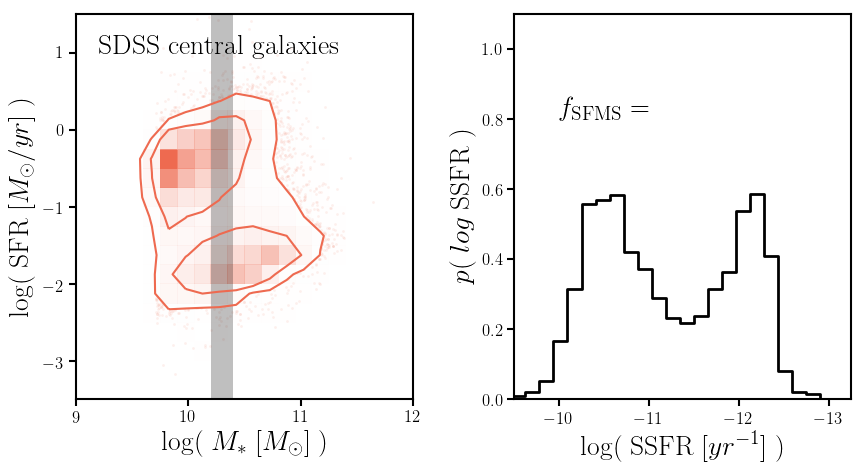
\includegraphics[width=0.9\textwidth]{figs/groupcat.png}
\caption{SDSS DR7 Group Catalog. Fitting of the SFMS.}
\label{fig:groupcat}
\end{center}
\end{figure}

\begin{figure}
\begin{center}
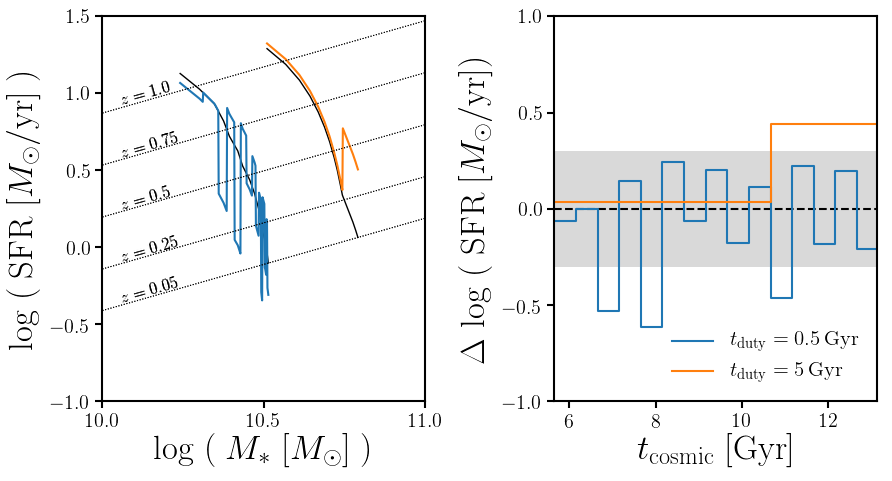
\includegraphics[width=0.9\textwidth]{figs/sfh_pedagogical.png}
\caption{Pedagogical figure that illustrates how star forming central galaxies in our model
evolve along the SFMS.}
\label{fig:sfh_model}
\end{center}
\end{figure}

%%%%%%%%%%%%%%%%%%%%%%%%%%%%%%%%%%%%%%%%%%%%%%%%%%%%%%%%%%%%%%%
% Acknowledgements
%%%%%%%%%%%%%%%%%%%%%%%%%%%%%%%%%%%%%%%%%%%%%%%%%%%%%%%%%%%%%%%
\section*{Acknowledgements}

%\bibliographystyle{yahapj}
\bibliography{centralMS}
\end{document}
